% Author: Seongjin Lee 
% Gyeongsang National University, Korea 
% 
% 2017-03-06
%

\documentclass[newPxFont,
%              sthlmFooter,
               nooffset]{beamer}
\usepackage{kotex}
\usetheme{boxes}


%\usepackage{../style/beamerthemesthlm}
%\hypersetup{pdfauthor={Seongjin Lee (insight@gnu.ac.kr)},
            %pdfsubject={Data Structure and Algorithm, Lecture Note},
            %pdfkeywords={Data Structure, Algorithm, Lecture, Note},
            %pdfmoddate={D: \pdfdate},
            %pdfcreator={Seongjin Lee}}

%\setbeamertemplate{footline}[text line]{%
%    \parbox{\linewidth}{\vspace*{-8pt} \insertsectionhead  \hfill\insertshortauthor\hfill\insertpagenumber}}
%\setbeamertemplate{navigation symbols}{}

\usepackage{tkz-graph}

\setbeamertemplate{blocks}[rounded]

\title{Data Structure and Algorithm}
\subtitle{MST Excercise}
\author[SJL]{Seongjin Lee}
\institute{\href{mailto:insight@gnu.ac.kr}{insight@gnu.ac.kr}\\\url{http://resourceful.github.io}\\Systems Research Lab.\\GNU}
\date{2017-03-06} 

\begin{document}
\beamertemplatenavigationsymbolsempty


%\frame[plain,t]{\titlepage} 

%\frame{\frametitle{Table of contents}\tableofcontents} 


\begin{frame}[t]
  \frametitle{Minimum Cost Spanning Tree Exercise}

  \begin{center}
    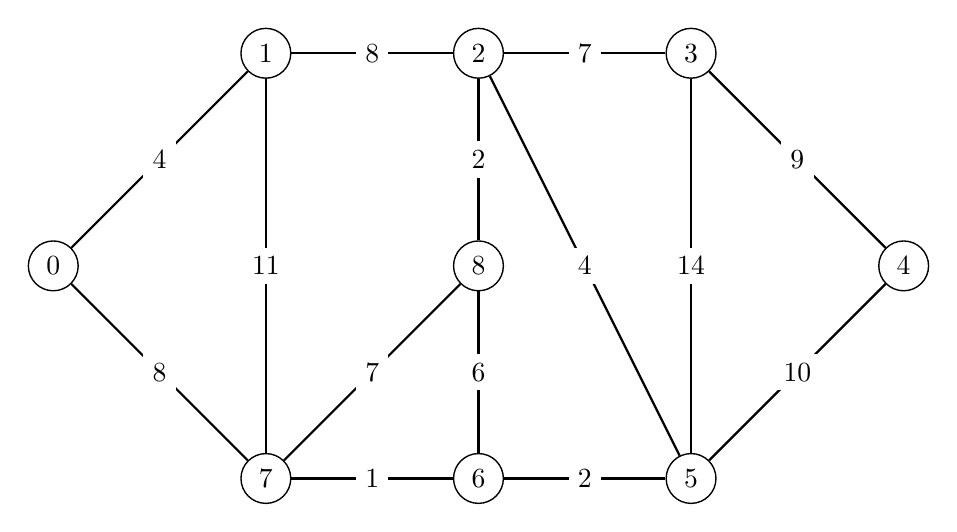
\begin{tikzpicture}
    \GraphInit[vstyle=Normal]
    \Vertex{0}\SetGraphUnit{2.7}
    \NOEA(0){1}
    \SOEA(0){7}
    \EA(1){2}
    \EA(2){3}
    \SOEA(3){4}
    \EA(7){6}
    \EA(6){5}
    \NOEA(7){8}
    \Edges[label=4](0, 1)
    \Edges[label=8](1, 2)
    \Edges[label=11](1, 7)
    \Edges[label=7](2, 3)
    \Edges[label=4](2, 5)
    \Edges[label=9](3, 4)
    \Edges[label=14](3, 5)
    \Edges[label=10](4, 5)
    \Edges[label=2](5, 6)
    \Edges[label=1](6, 7)
    \Edges[label=6](6, 8)
    \Edges[label=8](7, 0)
    \Edges[label=7](7, 8)
    \Edges[label=2](8, 2)
   \end{tikzpicture}
  \end{center}

\end{frame}


\begin{frame}[t]
  \frametitle{Minimum Cost Spanning Tree Exercise}

  \begin{center}
    \begin{tikzpicture}
    \GraphInit[vstyle=Normal]
    \Vertex{0}\SetGraphUnit{2.7}
    \NOEA(0){1}
    \SOEA(0){7}
    \EA(1){2}
    \EA(2){3}
    \SOEA(3){4}
    \EA(7){6}
    \EA(6){5}
    \NOEA(7){8}

   \end{tikzpicture}
  \end{center}

\end{frame}

\begin{frame}[t]
  \frametitle{Minimum Cost Spanning Tree Exercise}

  \begin{center}
    \begin{tikzpicture}
    \GraphInit[vstyle=Normal]
    \Vertex{0}\SetGraphUnit{2.7}
    \NOEA(0){1}
    \SOEA(0){7}
    \EA(1){2}
    \EA(2){3}
    \SOEA(3){4}
    \EA(7){6}
    \EA(6){5}
    \NOEA(7){8}

   \end{tikzpicture}
  \end{center}

\end{frame}

\begin{frame}[t]
  \frametitle{Minimum Cost Spanning Tree Exercise}

  \begin{center}
    \begin{tikzpicture}
    \GraphInit[vstyle=Normal]
    \Vertex{0}\SetGraphUnit{2.7}
    \NOEA(0){1}
    \SOEA(0){7}
    \EA(1){2}
    \EA(2){3}
    \SOEA(3){4}
    \EA(7){6}
    \EA(6){5}
    \NOEA(7){8}

   \end{tikzpicture}
  \end{center}

\end{frame}


\begin{frame}[t]
  \frametitle{Minimum Cost Spanning Tree Exercise}

  \begin{center}
    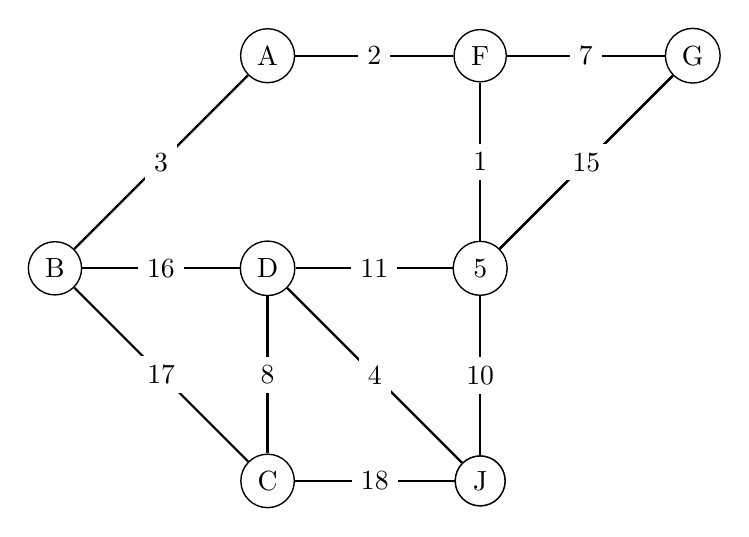
\begin{tikzpicture}
    \GraphInit[vstyle=Normal]\SetGraphUnit{2.7}
      \Vertex{A}
      \SOWE(A){B}
      \SOEA(B){C}
      \SO(A){D}
      \SOEA(D){I}
      \EA(D){E}
      \EA(A){F}
      \EA(F){G}
      \EA(D){H}
      \SO(H){J}
      \Edges[label=3](A,B)
      \Edges[label=2](A,F)
      \Edges[label=7](F,G)
      \Edges[label=1](F,E)
      \Edges[label=6](E,G)
      \Edges[label=15](G,H)
      \Edges[label=5](E,H)
      \Edges[label=13](H,J)
      \Edges[label=12](H,I)
      \Edges[label=10](E,I)
      \Edges[label=11](D,E)
      \Edges[label=4](D,I)
      \Edges[label=8](D,C)
      \Edges[label=18](C,I)
      \Edges[label=17](B,C)
      \Edges[label=16](B,D)
   \end{tikzpicture}
  \end{center}

\end{frame}

\begin{frame}[t]
  \frametitle{Minimum Cost Spanning Tree Exercise}

  \begin{center}
    \begin{tikzpicture}
    \GraphInit[vstyle=Normal]\SetGraphUnit{2.7}
      \Vertex{A}
      \SOWE(A){B}
      \SOEA(B){C}
      \SO(A){D}
      \SOEA(D){I}
      \EA(D){E}
      \EA(A){F}
      \EA(F){G}
      \EA(D){H}
      \SO(H){J}

   \end{tikzpicture}
  \end{center}

\end{frame}


\begin{frame}[t]
  \frametitle{Minimum Cost Spanning Tree Exercise}

  \begin{center}
    \begin{tikzpicture}
    \GraphInit[vstyle=Normal]\SetGraphUnit{2.7}
      \Vertex{A}
      \SOWE(A){B}
      \SOEA(B){C}
      \SO(A){D}
      \SOEA(D){I}
      \EA(D){E}
      \EA(A){F}
      \EA(F){G}
      \EA(D){H}
      \SO(H){J}

   \end{tikzpicture}
  \end{center}

\end{frame}


\begin{frame}[t]
  \frametitle{Minimum Cost Spanning Tree Exercise}

  \begin{center}
    \begin{tikzpicture}
    \GraphInit[vstyle=Normal]\SetGraphUnit{2.7}
      \Vertex{A}
      \SOWE(A){B}
      \SOEA(B){C}
      \SO(A){D}
      \SOEA(D){I}
      \EA(D){E}
      \EA(A){F}
      \EA(F){G}
      \EA(D){H}
      \SO(H){J}

   \end{tikzpicture}
  \end{center}

\end{frame}


\end{document}
